\documentclass{article}

\usepackage[utf8]{inputenc}
\usepackage{enumitem}
\usepackage{multirow}
\usepackage{xcolor}
\usepackage[T1]{fontenc}
% \usepackage[french]{babel}
\usepackage{hyperref}
\usepackage{amssymb}
\usepackage{mathtools}
\usepackage{ntheorem}
\usepackage{amsmath}
\usepackage{amssymb}
\usepackage[ a4paper, hmargin={2cm, 2cm}, vmargin={3cm, 3cm}]{geometry}
\usepackage{capt-of}
\usepackage{multicol}
\usepackage{mathpartir}

\usepackage[braket, qm]{qcircuit}
\usepackage{graphicx}

\usepackage{tikz}
\usetikzlibrary{angles,quotes}

\theoremstyle{plain}
\theorembodyfont{\normalfont}
\theoremseparator{~--}
\newtheorem{exo}{Exercise}[section]
\newtheorem{ans}{Answer}[section]
\newtheorem{lemma}{Lemma}[section]

\newcommand{\norm}[1]{\left\lVert#1\right\rVert}

\usepackage{hyperref}
\hypersetup{
    colorlinks,
    citecolor=black,
    filecolor=black,
    linkcolor=blue,
    urlcolor=blue
}

\usepackage{xcolor}

\definecolor{codegreen}{rgb}{0,0.6,0}
\definecolor{codegray}{rgb}{0.5,0.5,0.5}
\definecolor{codepurple}{rgb}{0.58,0,0.82}

\usepackage{listings}
\lstdefinestyle{mystyle}{
    commentstyle=\color{codegreen},
    keywordstyle=\color{magenta},
    numberstyle=\tiny\color{codegray},
    stringstyle=\color{codepurple},
    basicstyle=\ttfamily\footnotesize,
    breakatwhitespace=false,
    breaklines=true,
    captionpos=b,
    keepspaces=true,
    numbers=left,
    numbersep=5pt,
    showspaces=false,
    showstringspaces=false,
    showtabs=false,
    tabsize=2
}
\lstset{style=mystyle}

\theoremstyle{plain}
\theorembodyfont{\normalfont}
\theoremseparator{~--}
\newtheorem*{proof}{Proof}
\newtheorem*{exam}{Example}
\renewcommand\qedsymbol{$\square$}


\title{$\lambda$-calculus}
\author{Valeran MAYTIE}
\date{}

\begin{document}
  \maketitle

  \tableofcontents

  \newpage
  \section{Presentation}

  \begin{itemize}
    \item 1935 (a theory of computable functions)

      Alonzo Church, attempt at formalizing computation
  \end{itemize}

  Functions:
  \begin{itemize}
    \item maths : $f : A \to B$ is a set of pairs
    \item programming : instruction to compute an output
  \end{itemize}

  \subsection{Definitions}

  We can define the set of $\lambda$-terms ($\Lambda$) with a grammar:
  \begin{align*}
    \Lambda :=&\; x, y, z ...         & (\text{variable}) \\
             |&\; \lambda. \Lambda    & (\text{functions}) \\
             |&\; \Lambda\; \Lambda   & (\text{application})
  \end{align*}

  The application is left associative: $(l_1\; l_2)\; l_3$.

  \paragraph{Notations} We can define some notations to simplify the syntax :

  \begin{center}
  \begin{tabular}{ c|c }
    Real $\lambda$-term & notations \\
    \hline
    $\lambda x_1.(\ldots(\lambda x_n. t)\ldots)$ & $\lambda x_1 \ldots
    \lambda x_n. t$ \\
    $(\ldots (t\; u_1)\ldots)$ & $t\;u_1 \ldots u_n$ \\
    $t\; u_1\; \ldots_; u_n$ & $t\; \vec{u}$ with $\vec u = u_1\; \ldots\; u_n$
  \end{tabular}
  \end{center}

  \exam We can define this $\lambda$-term:

  \begin{itemize}
    \item Identity : $I = \lambda x.\; x$
    \item Constant generator: $C_c = \lambda x.\; c$
    \item Distribution : $\lambda x\; y\; z.\; (x\;z)\; (y\;z)$
    \item What ? : $\delta = \lambda x.\;x\;x$
    \item $A = \lambda x\;y.\; y(x\;x\;y)$
    \item Fix point : $\Theta = A A$ 
  \end{itemize}


  \paragraph{Curryfication} Functions are curryfied (Haskell Curry)

  They are no cartesian product in the $\lambda$-calculus. So we can define :

  \begin{center}
  \begin{tabular}{l l l}
    $\bullet$ A function: & $(x, y)\mapsto t$ & $\lambda x\;y.\; t$ \\
    $\bullet$ An application & $f(x, y)$ & $f\; x\; y$
  \end{tabular}
  \end{center}


    There are several possibilities when reducing terms. We can draw these
  possibilities in the form of a graph like this one:

  \begin{center}
  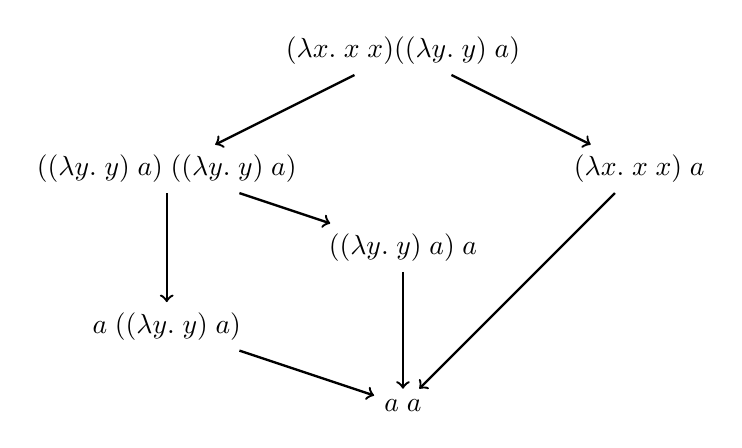
\begin{tikzpicture}[line width=0.3mm]
    \node(T1) at ( 0,  0) {$(\lambda x.\; x\;x)((\lambda y.\;y)\; a)$};
    \node(T2) at (-3, -1.5) {$((\lambda y.\;y)\; a)\;((\lambda y.\;y)\; a)$};
    \node(T3) at ( 3, -1.5) {$(\lambda x.\; x\;x)\;a$};
    \node(T4) at ( 0, -2.5) {$((\lambda y.\;y)\; a)\;a$};
    \node(T5) at (-3, -3.5) {$a\;((\lambda y.\;y)\;a)$};
    \node(T6) at ( 0, -4.5) {$a\;a$};

    \draw[->] (T1) edge (T2) (T2) edge (T4) (T4) edge (T6) (T3) edge (T6)
              (T2) edge (T5) (T5) edge (T6) (T1) edge (T3);
  \end{tikzpicture}
  \end{center}

  This raises the questions : \begin{itemize}
    \item Are some paths better than others ?
    \item Is there always a result in the ? Is it unique ?
  \end{itemize}

  \subsection{Normalization}

  A \textit{normal form} is a term that cannot be reduced anymore,
  formally : $N(t) = \neg \exists t', t \to t' $.

  \exam.

  \begin{tabular}{c|c}
    normal form & not normal form \\
    \hline
    $x$ & $(\lambda x.x)\; y$ \\
    $\lambda x.xy$ & $x\; ((\lambda y.y)\;(\lambda z.zx))$ \\
    $x (\lambda y.y)\;(\lambda z.zx)$ &
  \end{tabular}

  \vspace{0.5cm}

  If $t\to^* t'$ and $t'$ is normal, the term $t'$ is said to be a normal form
  of $t$. This defines our informal notion of a result of a term.

  Some terms do not have a normal form :

  \begin{align*}
    \Omega &= \delta\;\delta \\
          &= (\lambda x.xx)\; (\lambda x.xx) \\
          &\to (xx)\{\lambda x.xx\} \\
          &= x\{\lambda x.xx\}\;x\{\lambda x.xx\} \\
          &= (\lambda x.xx)\; (\lambda x.xx) \\
          &= \Omega
  \end{align*}

  \paragraph{Normalization properties} A term $t$ is :

  \begin{itemize}
    \item \textit{strongly normalizing} if every reduction sequence starting
      from $t$ eventually reaches a normal form :

      \[(\lambda xy.y)\;((\lambda z.z)\;(\lambda z.z))\]

    \item \textit{weakly normalizing}, or normalizable, if there is at least one
      reduction sequence starting from $t$ and reaching a normal form :

      \[(\lambda xy.y)\;((\lambda z.zz)\;(\lambda z.zz))\]
  \end{itemize}

  \subsection{Reduction strategies}

  The purpose of a reduction strategy is to determine a redex reduction order
  within a term. We have two well-known reduction orders :

  \begin{itemize}
    \item \textit{Normal order} : reduce the most external redex first. Apply
      functions without reducing the arguments
    \item \textit{Applicative order} : reduce the most internal redex first.
      Normalize the arguments before reducing the function application itself.
  \end{itemize}

  \exo normal order vs. applicative order.

  Compare normal order reduction and applicative order reduction of the
  following terms :

  \begin{enumerate}
    \item $(\lambda xy.x)\;z\;\Omega$
    \item $(\lambda x.xx)((\lambda y.y)\;z)$
    \item $(\lambda x.x(\lambda y.y)) (\lambda z.(\lambda a.aa)(z\;b))$
  \end{enumerate}

  In each case: does another order allow shorter sequences ?

  \textit{Answer}

  \begin{enumerate}
    \item Normal order
      \begin{align*}
        &(\lambda xy.x)\;z\;\Omega\\
        &\to (\lambda y.z)\; \Omega\\
        &\to z
      \end{align*}

      Applicative order
      \begin{align*}
        &(\lambda xy.x)\;z\;\Omega\\
        &\to (\lambda xy.x)\; \Omega\\
        &\to \ldots
      \end{align*}

      Normal order reduction is as short as possible.

    \item Normal order
      \begin{align*}
        &(\lambda x.xx)\;((\lambda y.y)\;z) \\
        &\to ((\lambda y.y)\; z)\;((\lambda y.y)\;z) \\
        &\to z ((\lambda y.y)\;z) \\
        &\to zz
      \end{align*}

      Applicative order

      \begin{align*}
        &(\lambda x.xx)\;((\lambda y.y)\;z) \\
        &\to (\lambda x.xx)\;z \\
        &\to zz
      \end{align*}

      Applicative order reduction is as short as possible.

    \item Reduction graph :
      \begin{center}
      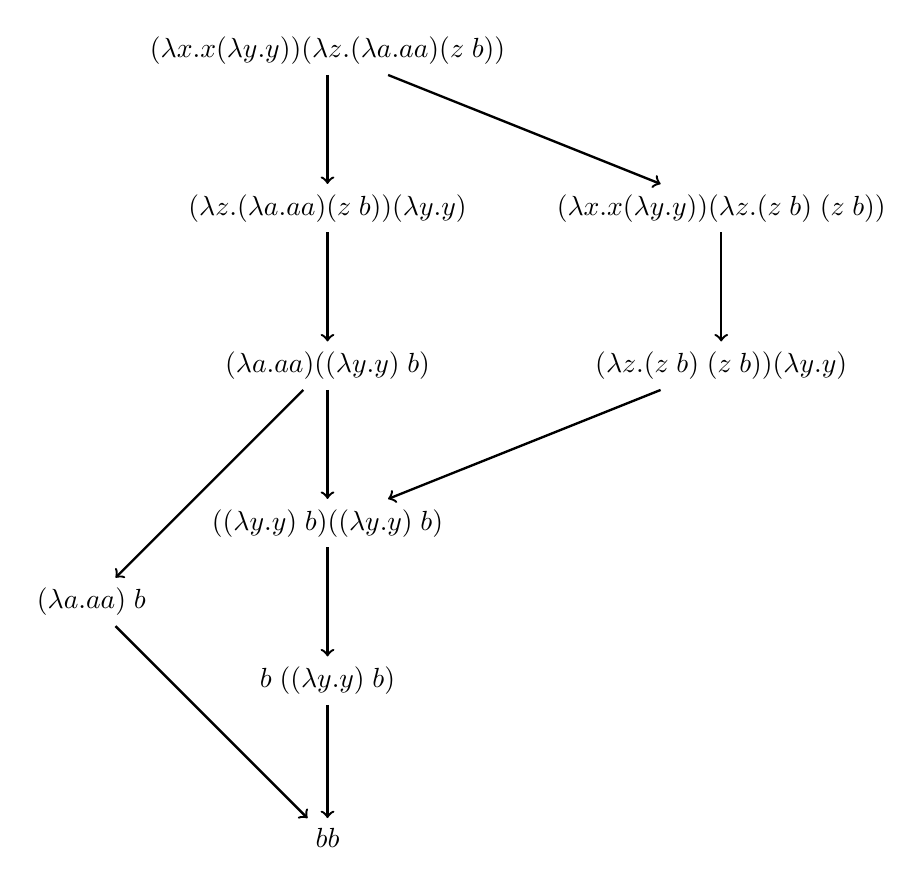
\begin{tikzpicture}[line width=0.3mm]
        \node(T1) at (0, 0) {$(\lambda x.x(\lambda y.y)) (\lambda z.(\lambda a.aa)(z\;b))$};
        \node(T2) at (0, -2) {$(\lambda z.(\lambda a.aa)(z\;b))(\lambda y.y)$};
        \node(T3) at (0, -4) {$(\lambda a.aa)((\lambda y.y)\;b)$};
        \node(T4) at (0, -6) {$((\lambda y.y)\;b)((\lambda y.y)\;b)$};
        \node(T5) at (0, -8) {$b\;((\lambda y.y)\;b)$};
        \node(T6) at (0, -10) {$bb$};

        \node(T7) at (5, -2) {$(\lambda x.x(\lambda y.y)) (\lambda z.(z\;b)\;(z\;b))$};
        \node(T8) at (5, -4) {$(\lambda z.(z\;b)\;(z\;b))(\lambda y.y)$};

        \node(T9) at (-3, -7) {$(\lambda a.aa)\;b$};

        \draw[->] (T1) edge (T2) (T2) edge (T3) (T3) edge (T4) (T4) edge (T5)
                  (T5) edge (T6)
                  (T1) edge (T7) (T7) edge (T8) (T8) edge (T4)
                  (T3) edge (T9) (T9) edge (T6);
      \end{tikzpicture}
      \end{center}

      The middle path is the normal order strategy, the right path is the
      applicative order and the left path is the shortest reduction.
  \end{enumerate}

  \paragraph{Normal order property} If a term $t$ does have a normal form the
  normal order reduction reaches this normal form.

  \subsection{Confluence}

  Confluence is a very useful concept to prove the uniqueness of a result of
  a calculation rule like beta-reduction. It says that if a term can be
  rewritten in more than one way, then there is always a way to revert to a
  common term

  Formally, the confluence is written
  like this: $\forall t\; t_1\; t_2, t \to^* t_1 \wedge t \to^* t_2 \Rightarrow
  \exists u, t_1 \to^* u \wedge t_2 \to^* u$

  We can draw the following diagram:

  \begin{center}
  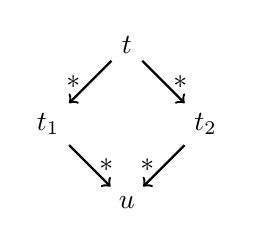
\begin{tikzpicture}[line width=0.3mm]
    \node(t) at (0, 0) {$t$};
    \node(t1) at (-1,-1) {$t_1$};
    \node(t2) at ( 1,-1) {$t_2$};
    \node(u) at ( 0,-2) {$u$};

    \draw[->] (t) edge node[pos=0.9, above] {$*$} (t1)
              (t) edge node[pos=0.9, above] {$*$} (t2)
              (t1) edge node[pos=0.9, above] {$*$} (u)
              (t2) edge node[pos=0.9, above] {$*$} (u);
  \end{tikzpicture}
  \end{center}

  A rewrite rule can have the \textit{diamond property}. In one rewriting step,
  it can always fall back on the same term in the second rewriting step.
  $\forall t\; t_1\; t_2, t \to t_1 \wedge t_2 \Rightarrow \exists u, t_1 \to u
  \wedge t_2 \to u$

  \begin{center}
  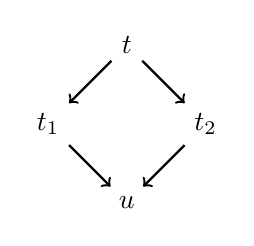
\begin{tikzpicture}[line width=0.3mm]
    \node(t) at (0, 0) {$t$};
    \node(t1) at (-1,-1) {$t_1$};
    \node(t2) at ( 1,-1) {$t_2$};
    \node(u) at ( 0,-2) {$u$};

    \draw[->] (t) edge (t1)
              (t) edge (t2)
              (t1) edge (u)
              (t2) edge (u);
  \end{tikzpicture}
  \end{center}

  \lemma The diamond property implies the confluence.

  \paragraph{proof}
  We can prove that by induction
  on $n + m$ with $n$ the number of steps of $t \to t_1$ and $m$ the number of
  steps of $t \to t_2$.

  \begin{itemize}
    \item $n + m = 0$, then $t = t_1 = t_2$, so $t \not \to t_1$ and $t \not \to
      t_2$ the property is true.

    \item $n + m + 1$ we assume that the diamond property implies the confluence
      on the condition that $t$ reduce to $t_1$ less that $n$ steps and $t$
      reduce to $t_2$ less that $m$ steps.

      \begin{center}
        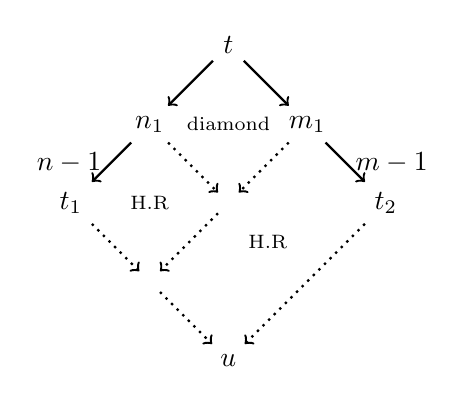
\begin{tikzpicture}[line width=0.3mm]
        \node(t) at (0, 0) {$t$};
        \node(n1) at (-1, -1) {$n_1$};
        \node(m1) at ( 1, -1) {$m_1$};
        \node(t1) at (-2, -2) {$t_1$};
        \node(t2) at ( 2, -2) {$t_2$};
        \node(u)  at ( 0, -4) {$u$};

        \node(nm)  at ( 0, -2) { };
        \node(t1n1)at ( -1, -3) { };

          \draw[->] (t) edge (n1)
                    (t) edge (m1)
                    (n1) edge node[above, left] {$n-1$} (t1)
                    (m1) edge node[above, right] {$m-1$} (t2);

        \draw[->, dotted] (n1) edge (nm) (m1) edge (nm);
        \draw[->, dotted] (t1) edge (t1n1) (nm) edge (t1n1);
        \draw[->, dotted] (t2) edge (u) (t1n1) edge (u);

        \node at (0, -1) {\scriptsize diamond};
        \node at (-1, -2) {\scriptsize H.R};
        \node at (0.5, -2.5) {\scriptsize H.R};

      \end{tikzpicture}
      \end{center}
  \end{itemize}
  \qedsymbol

  The $\beta$-reduction does not have the diamond property :

  \begin{center}
  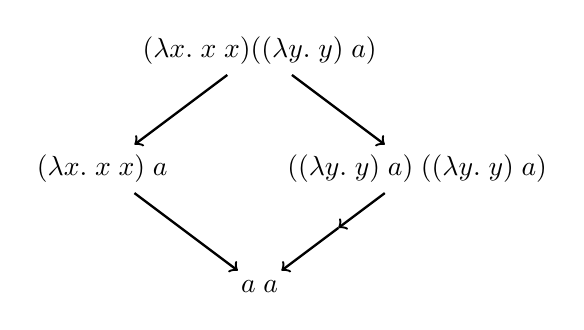
\begin{tikzpicture}[line width=0.3mm]
    \node(T1) at ( 0,  0) {$(\lambda x.\; x\;x)((\lambda y.\;y)\; a)$};
    \node(T3) at (-2, -1.5) {$(\lambda x.\; x\;x)\;a$};
    \node(T2) at ( 2, -1.5) {$((\lambda y.\;y)\; a)\;((\lambda y.\;y)\; a)$};
    \node(T6) at ( 0, -3) {$a\;a$};

    \draw[->] (T1) edge (T3) (T1) edge (T2) (T3) edge (T6)
      (T2) edge ( 1, -2.25)
      (1, -2.25) to (T6);
  \end{tikzpicture}
  \end{center}

  We can proof that the $\beta$-reduction is locally confluent, which is:
  $\forall t\; t_1\; t_2, t \to t_1 \wedge t \to t_2 \Rightarrow \exists u, t_1
  \to ^* u \wedge t_2 \to^* u$. It represents with this diagram :

  \begin{center}
  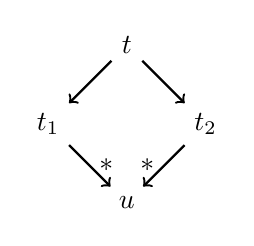
\begin{tikzpicture}[line width=0.3mm]
    \node(t) at (0, 0) {$t$};
    \node(t1) at (-1,-1) {$t_1$};
    \node(t2) at ( 1,-1) {$t_2$};
    \node(u) at ( 0,-2) {$u$};

    \draw[->] (t) edge (t1)
              (t) edge (t2)
              (t1) edge node[above, pos=0.9] {$*$} (u)
              (t2) edge node[above, pos=0.9] {$*$} (u);
  \end{tikzpicture}
  \end{center}

  But the local confluence does not imply the confluence, the Curry's counter
  example. This diagram is locally confluent, but it is not confluent.

  \begin{center}
  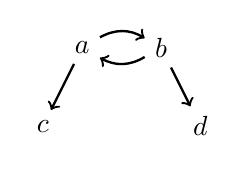
\begin{tikzpicture}[line width=0.3mm]
    \node(a) at (-0.5, 0) {$a$};
    \node(b) at (0.5,0) {$b$};

    \node(c) at (-1,-1) {$c$};
    \node(d) at ( 1,-1) {$d$};

    \draw[->] (a) edge[bend left] (b)
              (b) edge[bend left] (a)
              (a) edge (c)
              (b) edge (d);

  \end{tikzpicture}
  \end{center}

  The proof of confluence is therefore much more complicated than expected.
  We will present two possible proofs.

  \subsubsection{Parallel reduction}

  Parallel reduction proof consists of defining a relation
  $\rightrightarrows_\beta$ that is ``between'' $\to_\beta$ and $\to_\beta^*$.
  This relation need to have the diamond property. Because thanks to this we can
  prove the confluence of this new relation.

  We're going to start by defining the parallel reduction :

  \begin{mathpar}
    \inferrule*[Right=Id]{ }
              { x \\ \rightrightarrows_\beta \\ x} \\

    \inferrule*[Right=Abs]{t \\ \rightrightarrows_\beta \\ t'}
              {\lambda x.t \\ \rightrightarrows_\beta \\ \lambda x.t} \and
    \inferrule*[Right=App]{t_1 \rightrightarrows_\beta t_1' \\ t_2
      \rightrightarrows_\beta t_2' }
              {t_1\;t_2 \\ \rightrightarrows_\beta \\ t_1'\; t_2'} \\
    \inferrule*[Right=Red]{t \rightrightarrows_\beta t' \\ u
    \rightrightarrows_\beta u'}
        {(\lambda x. t) u \rightrightarrows_\beta t'\{x \leftarrow u'\}}
  \end{mathpar}

  \exam $(\lambda x.((\lambda y.y)\;(\lambda z.z))\;x)\;((\lambda w.w)\;a)$

  \begin{mathpar}
    \inferrule*{
      \inferrule*{
        \inferrule*{\inferrule*{ }{y \rightrightarrows_\beta y} \\
          \inferrule*{\inferrule*{ }{z \rightrightarrows_\beta z}}
            {\lambda z.z\rightrightarrows_\beta \lambda z.z}}
          {(\lambda y.y)\;(\lambda z.z)\rightrightarrows_\beta\lambda z.z}
        \\ \inferrule* { }{x\rightrightarrows_\beta x}}
      {(\lambda x.((\lambda y.y)\;(\lambda z.z))\;x)\rightrightarrows_\beta (\lambda z.z)\;x}
    \\
    \inferrule*{\inferrule*{ }{w \rightrightarrows_\beta w} \\
      \inferrule*{ }{a \rightrightarrows_\beta a}}
      {(\lambda w.w)a\rightrightarrows_\beta a}}
     {(\lambda x.((\lambda y.y)\;(\lambda z.z))\;x)\;((\lambda w.w)\;a) \rightrightarrows_\beta (\lambda z.z)\;a}
  \end{mathpar}

  \lemma \label{pid} $\forall t, t \rightrightarrows_\beta t$

  \textit{Proof}: We prove by induction on $t$:

  \begin{itemize}
    \item $t = x$ by definition of $\rightrightarrows_\beta$ we have $x
      \rightrightarrows_\beta a$.
    \item $t = t_1\; t_2$. We have this induction hypothesis $t_1
      \rightrightarrows_\beta t_1$ and $t_2 \rightrightarrows_\beta t_2$. So we
      have $t_1\; t_2 \rightrightarrows_\beta t_1\; t_2$
    \item $t = \lambda x.t_0$. We have this induction hypothesis $t_0
      \rightrightarrows_\beta t_0$. So we have $\lambda x.t_0
      \rightrightarrows_\beta \lambda x.t_0$.
  \end{itemize}
  \qedsymbol

  \lemma $\forall t t', t \to_\beta t' \Rightarrow t \rightrightarrows_\beta
  t'$\hspace{1cm} $\;\to_\beta \subseteq \rightrightarrows_\beta$

  \textit{Proof}: We prove by induction on $\to_\beta$

  \begin{itemize}
    \item Case $(\lambda x.t)\; u \to_\beta t \{x \leftarrow u\}$:

      \begin{mathpar}
        \inferrule*{
          \inferrule*[Left=Lemma-\ref{pid}]{ }{t \rightrightarrows_\beta t} \\
          \inferrule*[Right=Lemma-\ref{pid}]{ }{u \rightrightarrows_\beta u}
        }
          {(\lambda x.t)\; u \rightrightarrows_\beta t \{x \leftarrow u\}}
      \end{mathpar}
    \item Case $t_1\;t_2 \to_\beta t_1'\;t_2$ with $t_1 \to_\beta t_2$. With
      the induction hypothesis $t_1 \rightrightarrows_\beta t_1'$

      \begin{mathpar}
        \inferrule*{\inferrule*[Left=H.R]{ }{t_1\rightrightarrows_\beta t_1'}\\
          \inferrule*[Right=Lemma-\ref{pid}]{ }{t_2 \rightrightarrows_\beta t_2}}
          {t_1\;t_2 \rightrightarrows_\beta t_1'\;t_2}
      \end{mathpar}
    \item The other case are similar.
  \end{itemize}

  \lemma $\forall t t', t \rightrightarrows_\beta t' \Rightarrow t \to_\beta^*
  t'$ \hspace{1cm} $\rightrightarrows_\beta \subseteq \to_\beta^*$

  \textit{Proof}: by induction on $\rightrightarrows_\beta$

  \begin{itemize}
    \item Case $x \rightrightarrows_\beta x$. We have $x\to^0_\beta x$

    \item Case $\lambda x. u \rightrightarrows_\beta \lambda x. u'$ with $t
      \rightrightarrows_\beta t'$. We assume that $t \to_\beta^* t'$ (induction
      hypothesis). We can easily prove by recurrence on the length of
      $\to_\beta^*$, that we have well $\lambda x. t \to_\beta^* \lambda x.t'$

    \item The application rule is similar.

    \item Case $(\lambda x. t)\; u \rightrightarrows_\beta t'\{x \leftarrow
      u'\}$ with $t \rightrightarrows_\beta t'$ and $u \rightrightarrows_\beta
      u'$. Then we have $(\lambda x. t) u \to_\beta^* (\lambda x. t') u$ by
      induction hypothesis on $t$, $(\lambda x. t') u' \to_\beta^* (\lambda x.
      t') u'$ by induction hypothesis on $u$. And finally we have $(\lambda x.
      t') u' \to_\beta t'\{x\leftarrow u'\}$
  \end{itemize}
  \qedsymbol

  \paragraph{method of Tait and Martin-Löf} We want to proof that a relation has
  the diamond property

  \lemma If a relation $\to$ has the diamond property then $\to^*$ has the
  diamond property to.

  \textit{Proof} : We suppose that $\to$ has the diamond property [TODO]
  \qedsymbol

  \lemma If two relation  $\to$ and $\rightrightarrows$ are such that $\to
  \subseteq \rightrightarrows \subseteq \to^*$ then $\rightrightarrows^* =
  \to^*$.

  \textit{Proof}: From $\to \subseteq \rightrightarrows \subseteq \to^*$ we
  deduce $\to^* \subseteq \rightrightarrows^* \subseteq \to^{**}$. However we
  have $\to^* = \to^{**}$. Then $\to^* \subseteq \rightrightarrows
  \subseteq \to^*$ so we have $\rightrightarrows^* = \to^*$.\\
  \qedsymbol

  To proof that $\to^*$ has the diamond property we just need to show that
  $\rightrightarrows_\beta$ has the diamond property. To do this we need the
  following lemma :

  \lemma  \label{dia_iter}
  $a \rightrightarrows_\beta a' \wedge b \rightrightarrows_\beta b'
  \Rightarrow a\{x \leftarrow b\} \rightrightarrows_\beta a'\{x \leftarrow b\}$

  \textit{Proof}:
  By induction one the derivation $a \rightrightarrows_\beta a'$.

  \begin{itemize}
    \item Case $y \rightrightarrows_\beta y$
      \begin{itemize}
        \item If $x = y$, then $x\{x \leftarrow b\} = b \rightrightarrows_\beta
          b' = x\{x \leftarrow b'\}$

        \item If $x \not = y$, then $y\{x \leftarrow b\} = y
          \rightrightarrows_\beta y = y\{x \leftarrow b'\}$
      \end{itemize}

    \item Case $\lambda y. a_0 \rightrightarrows_\beta \lambda y.a_0'$ with $a_0
      \rightrightarrows_\beta a_0'$

      Then $(\lambda y.a_0)\{x\leftarrow b\} = \lambda y. a_0 \{x \leftarrow
      b\}$. By induction hypothesis we have $a_0\{x \leftarrow b\}
      \rightrightarrows_\beta a_0'\{x \leftarrow b'\}$.

      Therefore, we have $\lambda y.a_0\{x\leftarrow b\} \rightrightarrows_\beta
      \lambda y.a_0'\{x\leftarrow b'\} = (\lambda y.a_0')\{x\leftarrow b'\}$

    \item Case $a_1\; a_2 \rightrightarrows_\beta a_1'\;a_2'$ with $a_1
      \rightrightarrows_\beta a_1'$ and $a_2 \rightrightarrows_\beta a_2'$.

      It is similar to the case above.

    \item Case $(\lambda x. a_1)\;a_2\rightrightarrows_\beta (\lambda x.a_1')
      a_2'$ with $a_1 \rightrightarrows_\beta a_1'$ and $a_2
      \rightrightarrows_\beta a_2'$.

      Then $((\lambda y. a_1)a_2)\{x \leftarrow b\} = (\lambda y. a_1\{x
      \leftarrow b\})a_2\{x \leftarrow b\}$.

      By the induction hypothesis we have $a_1\{x \leftarrow b\}
      \rightrightarrows_\beta a_1'\{x \leftarrow b'\}$ and $a_2\{x \leftarrow
      b\} \rightrightarrows_\beta a_2'\{x \leftarrow b'\}$.

      Therefore $(\lambda y. a_1\{x\leftarrow b\})(a_2\{\leftarrow b\})
      \rightrightarrows_\beta (a_1'\{x \leftarrow b'\}\{y \leftarrow a_2'\{x
      \leftarrow b'\}\}$. Thanks to the substitution lemma-\ref{exo:commsubst}

  \end{itemize}
  \qedsymbol

  \lemma $\rightrightarrows_\beta$ has the diamond property.
    $\forall t\; s\; r, t \rightrightarrows_\beta s \wedge t \rightrightarrows_\beta
    r \Rightarrow \exists u, s \rightrightarrows_\beta u \wedge r
    \rightrightarrows_\beta u$.

  \textit{Proof}: By induction on the derivation of $t\rightrightarrows_\beta
  re$.

  \begin{itemize}
    \item Case $x \rightrightarrows_\beta x$. Then $s = x$ so we can take $u =
      x$.

    \item Case $\lambda x.t_0 \rightrightarrows_\beta \lambda x. r_0$ with
      $t_0 \rightrightarrows_\beta r_0$. Then $s = \lambda x. s_0$ with
      $t_0 \rightrightarrows_\beta s_0$.

      By induction hypothesis we have $u_0$ such that $s_0
      \rightrightarrows_\beta u_0$ and $r_0 \rightrightarrows_\beta u_0$.

      Therefore, $\lambda x. s_0 \rightrightarrows_\beta \lambda x. u_0$ And
      $\lambda x. r_0 \rightrightarrows_\beta \lambda x. u_0$

    \item Case $t_1\;t_2 \rightrightarrows_\beta r_1\; r_2$ with $t_1
      \rightrightarrows_\beta r_1$ and $t_2 \rightrightarrows_\beta r_2$.
      Two case for $t_1\;t_2 \rightrightarrows_\beta s_0$:

      \begin{itemize}
        \item if $s = s_1\;s_2$ with $t_1 \rightrightarrows_\beta s_1$ and $t_2
          \rightrightarrows_\beta s_2$ by induction hypothesis there are $u_1$
          and $u_2$ such that $s_1 \rightrightarrows_\beta u_1$, $r_1
          \rightrightarrows_\beta u_1$ and $s_2 \rightrightarrows_\beta u_2$,
          $r_2 \rightrightarrows_\beta u_2$, therefore $s_1s_2
          \rightrightarrows_\beta u_1u_2$ and $r_1r_2
          \rightrightarrows_\beta u_1u_2$.

        \item if $s = s_1\{x \leftarrow s_2\}$ with $t_1 = \lambda x.t_1$ and
          $t_1 \rightrightarrows_\beta s_1$ and $t_2 \rightrightarrows_\beta
          s_2$, then $r_1 = \lambda x.r_1$ with $t_1' \rightrightarrows_\beta
          r_1'$ and by induction hypothesis there are $u_1$ and $u_2$ such that
          $s_1 \rightrightarrows_\beta u_1$ and $r_1'\rightrightarrows_\beta
          u_1$ and $s_2 \rightrightarrows_\beta u_2$ and $r_2
          \rightrightarrows_\beta u_2$.

          Therefore, $(\lambda x.r_1')r_2 \rightrightarrows_\beta u_1\{
            x \leftarrow s_2\}$. And we conclude by the lemma-\ref{dia_iter}
      \end{itemize}

    \item The last case is almost the same.
  \end{itemize}
  \qedsymbol

  \subsubsection{Strip lemma}

  \subsubsection{Church-Rosser theorem}

  If $t_1 =_\beta t_2$ the there is $u$ such that $t_1 \to_\beta^* u$ and $t_2
  \to_\beta^* u$

  Consequences :

  \begin{itemize}
    \item if $t$ has a normal form $n$ then $t \to_\beta^* n$

    \item any $\lambda$-term can has only one normal form

    \item if two normal form $n$ and $m$ are syntactically different, then $n
      \not =_\beta m$.
  \end{itemize}



  \section{Reduction strategies}

  There are several possibilities when reducing terms. We can draw these
  possibilities in the form of a graph like this one:

  \begin{center}
  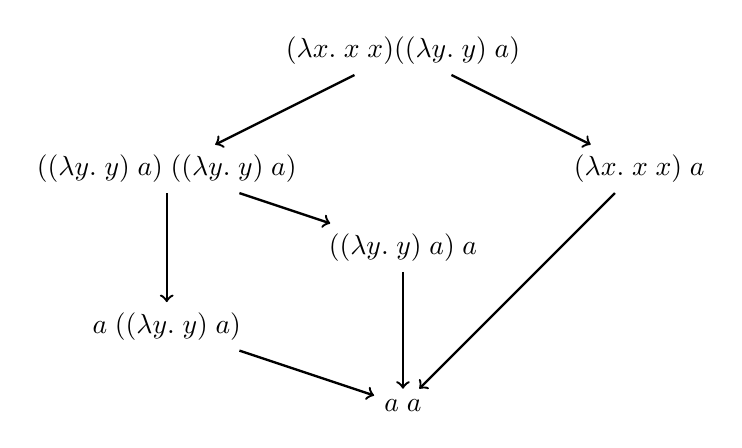
\begin{tikzpicture}[line width=0.3mm]
    \node(T1) at ( 0,  0) {$(\lambda x.\; x\;x)((\lambda y.\;y)\; a)$};
    \node(T2) at (-3, -1.5) {$((\lambda y.\;y)\; a)\;((\lambda y.\;y)\; a)$};
    \node(T3) at ( 3, -1.5) {$(\lambda x.\; x\;x)\;a$};
    \node(T4) at ( 0, -2.5) {$((\lambda y.\;y)\; a)\;a$};
    \node(T5) at (-3, -3.5) {$a\;((\lambda y.\;y)\;a)$};
    \node(T6) at ( 0, -4.5) {$a\;a$};

    \draw[->] (T1) edge (T2) (T2) edge (T4) (T4) edge (T6) (T3) edge (T6)
              (T2) edge (T5) (T5) edge (T6) (T1) edge (T3);
  \end{tikzpicture}
  \end{center}

  This raises the questions : \begin{itemize}
    \item Are some paths better than others ?
    \item Is there always a result in the ? Is it unique ?
  \end{itemize}

  \subsection{Normalization}

  A \textit{normal form} is a term that cannot be reduced anymore,
  formally : $N(t) = \neg \exists t', t \to t' $.

  \exam.

  \begin{tabular}{c|c}
    normal form & not normal form \\
    \hline
    $x$ & $(\lambda x.x)\; y$ \\
    $\lambda x.xy$ & $x\; ((\lambda y.y)\;(\lambda z.zx))$ \\
    $x (\lambda y.y)\;(\lambda z.zx)$ &
  \end{tabular}

  \vspace{0.5cm}

  If $t\to^* t'$ and $t'$ is normal, the term $t'$ is said to be a normal form
  of $t$. This defines our informal notion of a result of a term.

  Some terms do not have a normal form :

  \begin{align*}
    \Omega &= \delta\;\delta \\
          &= (\lambda x.xx)\; (\lambda x.xx) \\
          &\to (xx)\{\lambda x.xx\} \\
          &= x\{\lambda x.xx\}\;x\{\lambda x.xx\} \\
          &= (\lambda x.xx)\; (\lambda x.xx) \\
          &= \Omega
  \end{align*}

  \paragraph{Normalization properties} A term $t$ is :

  \begin{itemize}
    \item \textit{strongly normalizing} if every reduction sequence starting
      from $t$ eventually reaches a normal form :

      \[(\lambda xy.y)\;((\lambda z.z)\;(\lambda z.z))\]

    \item \textit{weakly normalizing}, or normalizable, if there is at least one
      reduction sequence starting from $t$ and reaching a normal form :

      \[(\lambda xy.y)\;((\lambda z.zz)\;(\lambda z.zz))\]
  \end{itemize}

  \subsection{Reduction strategies}

  The purpose of a reduction strategy is to determine a redex reduction order
  within a term. We have two well-known reduction orders :

  \begin{itemize}
    \item \textit{Normal order} : reduce the most external redex first. Apply
      functions without reducing the arguments
    \item \textit{Applicative order} : reduce the most internal redex first.
      Normalize the arguments before reducing the function application itself.
  \end{itemize}

  \exo normal order vs. applicative order.

  Compare normal order reduction and applicative order reduction of the
  following terms :

  \begin{enumerate}
    \item $(\lambda xy.x)\;z\;\Omega$
    \item $(\lambda x.xx)((\lambda y.y)\;z)$
    \item $(\lambda x.x(\lambda y.y)) (\lambda z.(\lambda a.aa)(z\;b))$
  \end{enumerate}

  In each case: does another order allow shorter sequences ?

  \textit{Answer}

  \begin{enumerate}
    \item Normal order
      \begin{align*}
        &(\lambda xy.x)\;z\;\Omega\\
        &\to (\lambda y.z)\; \Omega\\
        &\to z
      \end{align*}

      Applicative order
      \begin{align*}
        &(\lambda xy.x)\;z\;\Omega\\
        &\to (\lambda xy.x)\; \Omega\\
        &\to \ldots
      \end{align*}

      Normal order reduction is as short as possible.

    \item Normal order
      \begin{align*}
        &(\lambda x.xx)\;((\lambda y.y)\;z) \\
        &\to ((\lambda y.y)\; z)\;((\lambda y.y)\;z) \\
        &\to z ((\lambda y.y)\;z) \\
        &\to zz
      \end{align*}

      Applicative order

      \begin{align*}
        &(\lambda x.xx)\;((\lambda y.y)\;z) \\
        &\to (\lambda x.xx)\;z \\
        &\to zz
      \end{align*}

      Applicative order reduction is as short as possible.

    \item Reduction graph :
      \begin{center}
      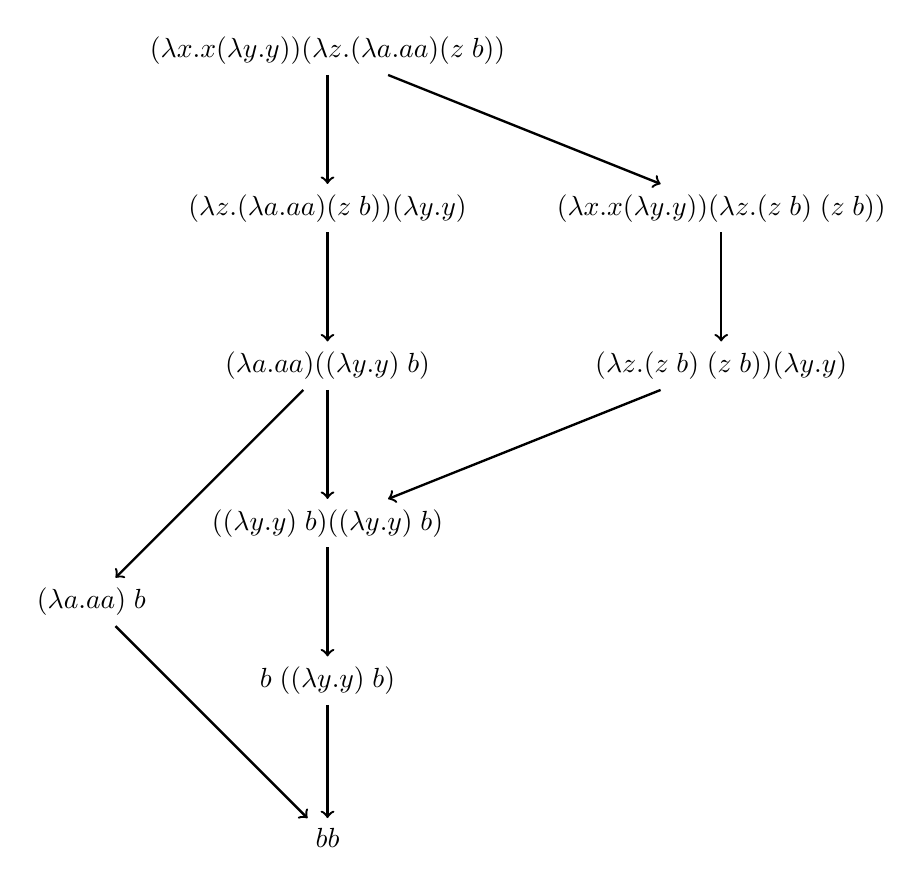
\begin{tikzpicture}[line width=0.3mm]
        \node(T1) at (0, 0) {$(\lambda x.x(\lambda y.y)) (\lambda z.(\lambda a.aa)(z\;b))$};
        \node(T2) at (0, -2) {$(\lambda z.(\lambda a.aa)(z\;b))(\lambda y.y)$};
        \node(T3) at (0, -4) {$(\lambda a.aa)((\lambda y.y)\;b)$};
        \node(T4) at (0, -6) {$((\lambda y.y)\;b)((\lambda y.y)\;b)$};
        \node(T5) at (0, -8) {$b\;((\lambda y.y)\;b)$};
        \node(T6) at (0, -10) {$bb$};

        \node(T7) at (5, -2) {$(\lambda x.x(\lambda y.y)) (\lambda z.(z\;b)\;(z\;b))$};
        \node(T8) at (5, -4) {$(\lambda z.(z\;b)\;(z\;b))(\lambda y.y)$};

        \node(T9) at (-3, -7) {$(\lambda a.aa)\;b$};

        \draw[->] (T1) edge (T2) (T2) edge (T3) (T3) edge (T4) (T4) edge (T5)
                  (T5) edge (T6)
                  (T1) edge (T7) (T7) edge (T8) (T8) edge (T4)
                  (T3) edge (T9) (T9) edge (T6);
      \end{tikzpicture}
      \end{center}

      The middle path is the normal order strategy, the right path is the
      applicative order and the left path is the shortest reduction.
  \end{enumerate}

  \paragraph{Normal order property} If a term $t$ does have a normal form the
  normal order reduction reaches this normal form.

  \subsection{Confluence}

  Confluence is a very useful concept to prove the uniqueness of a result of
  a calculation rule like beta-reduction. It says that if a term can be
  rewritten in more than one way, then there is always a way to revert to a
  common term

  Formally, the confluence is written
  like this: $\forall t\; t_1\; t_2, t \to^* t_1 \wedge t \to^* t_2 \Rightarrow
  \exists u, t_1 \to^* u \wedge t_2 \to^* u$

  We can draw the following diagram:

  \begin{center}
  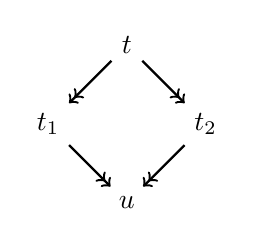
\begin{tikzpicture}[line width=0.3mm]
    \node(t) at (0, 0) {$t$};
    \node(t1) at (-1,-1) {$t_1$};
    \node(t2) at ( 1,-1) {$t_2$};
    \node(u) at ( 0,-2) {$u$};

    \draw[->>](t)  edge (t1)
              (t)  edge (t2)
              (t1) edge (u)
              (t2) edge (u);
  \end{tikzpicture}
  \end{center}

  A rewrite rule can have the \textit{diamond property}. In one rewriting step,
  it can always fall back on the same term in the second rewriting step.
  $\forall t\; t_1\; t_2, t \to t_1 \wedge t_2 \Rightarrow \exists u, t_1 \to u
  \wedge t_2 \to u$

  \begin{center}
  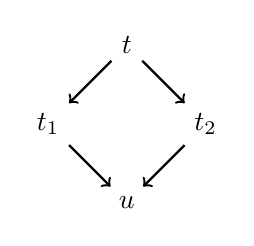
\begin{tikzpicture}[line width=0.3mm]
    \node(t) at (0, 0) {$t$};
    \node(t1) at (-1,-1) {$t_1$};
    \node(t2) at ( 1,-1) {$t_2$};
    \node(u) at ( 0,-2) {$u$};

    \draw[->] (t) edge (t1)
              (t) edge (t2)
              (t1) edge (u)
              (t2) edge (u);
  \end{tikzpicture}
  \end{center}

  \lemma The diamond property implies the confluence.

  \paragraph{proof}
  We can prove that by induction
  on $n + m$ with $n$ the number of steps of $t \to t_1$ and $m$ the number of
  steps of $t \to t_2$.

  \begin{itemize}
    \item $n + m = 0$, then $t = t_1 = t_2$, so $t \not \to t_1$ and $t \not \to
      t_2$ the property is true.

    \item $n + m + 1$ we assume that the diamond property implies the confluence
      on the condition that $t$ reduce to $t_1$ less that $n$ steps and $t$
      reduce to $t_2$ less that $m$ steps.

      \begin{center}
        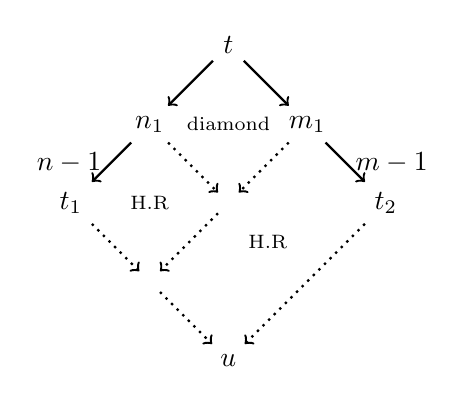
\begin{tikzpicture}[line width=0.3mm]
        \node(t) at (0, 0) {$t$};
        \node(n1) at (-1, -1) {$n_1$};
        \node(m1) at ( 1, -1) {$m_1$};
        \node(t1) at (-2, -2) {$t_1$};
        \node(t2) at ( 2, -2) {$t_2$};
        \node(u)  at ( 0, -4) {$u$};

        \node(nm)  at ( 0, -2) { };
        \node(t1n1)at ( -1, -3) { };

          \draw[->] (t) edge (n1)
                    (t) edge (m1)
                    (n1) edge node[above, left] {$n-1$} (t1)
                    (m1) edge node[above, right] {$m-1$} (t2);

        \draw[->, dotted] (n1) edge (nm) (m1) edge (nm);
        \draw[->, dotted] (t1) edge (t1n1) (nm) edge (t1n1);
        \draw[->, dotted] (t2) edge (u) (t1n1) edge (u);

        \node at (0, -1) {\scriptsize diamond};
        \node at (-1, -2) {\scriptsize H.R};
        \node at (0.5, -2.5) {\scriptsize H.R};

      \end{tikzpicture}
      \end{center}
  \end{itemize}
  \qedsymbol

  The $\beta$-reduction does not have the diamond property :

  \begin{center}
  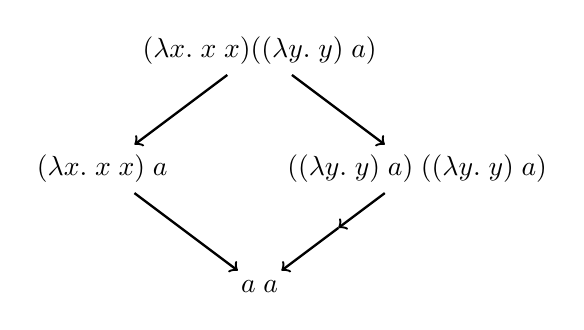
\begin{tikzpicture}[line width=0.3mm]
    \node(T1) at ( 0,  0) {$(\lambda x.\; x\;x)((\lambda y.\;y)\; a)$};
    \node(T3) at (-2, -1.5) {$(\lambda x.\; x\;x)\;a$};
    \node(T2) at ( 2, -1.5) {$((\lambda y.\;y)\; a)\;((\lambda y.\;y)\; a)$};
    \node(T6) at ( 0, -3) {$a\;a$};

    \draw[->] (T1) edge (T3) (T1) edge (T2) (T3) edge (T6)
      (T2) edge ( 1, -2.25)
      (1, -2.25) to (T6);
  \end{tikzpicture}
  \end{center}

  We can proof that the $\beta$-reduction is locally confluent, which is:
  $\forall t\; t_1\; t_2, t \to t_1 \wedge t \to t_2 \Rightarrow \exists u, t_1
  \to ^* u \wedge t_2 \to^* u$. It represents with this diagram :

  \begin{center}
  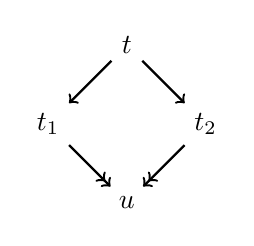
\begin{tikzpicture}[line width=0.3mm]
    \node(t) at (0, 0) {$t$};
    \node(t1) at (-1,-1) {$t_1$};
    \node(t2) at ( 1,-1) {$t_2$};
    \node(u) at ( 0,-2) {$u$};

    \draw[->] (t) edge (t1)
              (t) edge (t2);
    \draw[->>] (t1) edge (u)
               (t2) edge (u);
  \end{tikzpicture}
  \end{center}

  But the local confluence does not imply the confluence, the Curry's counter
  example. This diagram is locally confluent, but it is not confluent.

  \begin{center}
  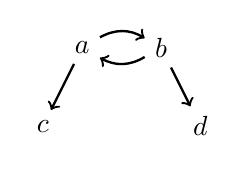
\begin{tikzpicture}[line width=0.3mm]
    \node(a) at (-0.5, 0) {$a$};
    \node(b) at (0.5,0) {$b$};

    \node(c) at (-1,-1) {$c$};
    \node(d) at ( 1,-1) {$d$};

    \draw[->] (a) edge[bend left] (b)
              (b) edge[bend left] (a)
              (a) edge (c)
              (b) edge (d);

  \end{tikzpicture}
  \end{center}

  The proof of confluence is therefore much more complicated than expected.
  We will present two possible proofs.

  \subsubsection{Parallel reduction}

  Parallel reduction proof consists of defining a relation
  $\rightrightarrows_\beta$ that is ``between'' $\to_\beta$ and $\to_\beta^*$.
  This relation need to have the diamond property. Because thanks to this we can
  prove the confluence of this new relation.

  We're going to start by defining the parallel reduction :

  \begin{mathpar}
    \inferrule*[Right=Id]{ }
              { x \\ \rightrightarrows_\beta \\ x} \\

    \inferrule*[Right=Abs]{t \\ \rightrightarrows_\beta \\ t'}
              {\lambda x.t \\ \rightrightarrows_\beta \\ \lambda x.t} \and
    \inferrule*[Right=App]{t_1 \rightrightarrows_\beta t_1' \\ t_2
      \rightrightarrows_\beta t_2' }
              {t_1\;t_2 \\ \rightrightarrows_\beta \\ t_1'\; t_2'} \\
    \inferrule*[Right=Red]{t \rightrightarrows_\beta t' \\ u
    \rightrightarrows_\beta u'}
        {(\lambda x. t) u \rightrightarrows_\beta t'\{x \leftarrow u'\}}
  \end{mathpar}

  \exam $(\lambda x.((\lambda y.y)\;(\lambda z.z))\;x)\;((\lambda w.w)\;a)$

  \begin{mathpar}
    \inferrule*{
      \inferrule*{
        \inferrule*{\inferrule*{ }{y \rightrightarrows_\beta y} \\
          \inferrule*{\inferrule*{ }{z \rightrightarrows_\beta z}}
            {\lambda z.z\rightrightarrows_\beta \lambda z.z}}
          {(\lambda y.y)\;(\lambda z.z)\rightrightarrows_\beta\lambda z.z}
        \\ \inferrule* { }{x\rightrightarrows_\beta x}}
      {(\lambda x.((\lambda y.y)\;(\lambda z.z))\;x)\rightrightarrows_\beta (\lambda z.z)\;x}
    \\
    \inferrule*{\inferrule*{ }{w \rightrightarrows_\beta w} \\
      \inferrule*{ }{a \rightrightarrows_\beta a}}
      {(\lambda w.w)a\rightrightarrows_\beta a}}
     {(\lambda x.((\lambda y.y)\;(\lambda z.z))\;x)\;((\lambda w.w)\;a) \rightrightarrows_\beta (\lambda z.z)\;a}
  \end{mathpar}

  \lemma \label{pid} $\forall t, t \rightrightarrows_\beta t$

  \textit{Proof}: We prove by induction on $t$:

  \begin{itemize}
    \item $t = x$ by definition of $\rightrightarrows_\beta$ we have $x
      \rightrightarrows_\beta a$.
    \item $t = t_1\; t_2$. We have this induction hypothesis $t_1
      \rightrightarrows_\beta t_1$ and $t_2 \rightrightarrows_\beta t_2$. So we
      have $t_1\; t_2 \rightrightarrows_\beta t_1\; t_2$
    \item $t = \lambda x.t_0$. We have this induction hypothesis $t_0
      \rightrightarrows_\beta t_0$. So we have $\lambda x.t_0
      \rightrightarrows_\beta \lambda x.t_0$.
  \end{itemize}
  \qedsymbol

  \lemma $\forall t t', t \to_\beta t' \Rightarrow t \rightrightarrows_\beta
  t'$\hspace{1cm} $\;\to_\beta \subseteq \rightrightarrows_\beta$

  \textit{Proof}: We prove by induction on $\to_\beta$

  \begin{itemize}
    \item Case $(\lambda x.t)\; u \to_\beta t \{x \leftarrow u\}$:

      \begin{mathpar}
        \inferrule*{
          \inferrule*[Left=Lemma-\ref{pid}]{ }{t \rightrightarrows_\beta t} \\
          \inferrule*[Right=Lemma-\ref{pid}]{ }{u \rightrightarrows_\beta u}
        }
          {(\lambda x.t)\; u \rightrightarrows_\beta t \{x \leftarrow u\}}
      \end{mathpar}
    \item Case $t_1\;t_2 \to_\beta t_1'\;t_2$ with $t_1 \to_\beta t_2$. With
      the induction hypothesis $t_1 \rightrightarrows_\beta t_1'$

      \begin{mathpar}
        \inferrule*{\inferrule*[Left=H.R]{ }{t_1\rightrightarrows_\beta t_1'}\\
          \inferrule*[Right=Lemma-\ref{pid}]{ }{t_2 \rightrightarrows_\beta t_2}}
          {t_1\;t_2 \rightrightarrows_\beta t_1'\;t_2}
      \end{mathpar}
    \item The other case are similar.
  \end{itemize}

  \lemma $\forall t t', t \rightrightarrows_\beta t' \Rightarrow t \to_\beta^*
  t'$ \hspace{1cm} $\rightrightarrows_\beta \subseteq \to_\beta^*$

  \textit{Proof}: by induction on $\rightrightarrows_\beta$

  \begin{itemize}
    \item Case $x \rightrightarrows_\beta x$. We have $x\to^0_\beta x$

    \item Case $\lambda x. u \rightrightarrows_\beta \lambda x. u'$ with $t
      \rightrightarrows_\beta t'$. We assume that $t \to_\beta^* t'$ (induction
      hypothesis). We can easily prove by recurrence on the length of
      $\to_\beta^*$, that we have well $\lambda x. t \to_\beta^* \lambda x.t'$

    \item The application rule is similar.

    \item Case $(\lambda x. t)\; u \rightrightarrows_\beta t'\{x \leftarrow
      u'\}$ with $t \rightrightarrows_\beta t'$ and $u \rightrightarrows_\beta
      u'$. Then we have $(\lambda x. t) u \to_\beta^* (\lambda x. t') u$ by
      induction hypothesis on $t$, $(\lambda x. t') u' \to_\beta^* (\lambda x.
      t') u'$ by induction hypothesis on $u$. And finally we have $(\lambda x.
      t') u' \to_\beta t'\{x\leftarrow u'\}$
  \end{itemize}
  \qedsymbol

  \paragraph{method of Tait and Martin-Löf} We want to proof that a relation has
  the diamond property

  \lemma If a relation $\to$ has the diamond property then $\to^*$ has the
  diamond property to.

  \textit{Proof} : We suppose that $\to$ has the diamond property [TODO]
  \qedsymbol

  \lemma If two relation  $\to$ and $\rightrightarrows$ are such that $\to
  \subseteq \rightrightarrows \subseteq \to^*$ then $\rightrightarrows^* =
  \to^*$.

  \textit{Proof}: From $\to \subseteq \rightrightarrows \subseteq \to^*$ we
  deduce $\to^* \subseteq \rightrightarrows^* \subseteq \to^{**}$. However we
  have $\to^* = \to^{**}$. Then $\to^* \subseteq \rightrightarrows
  \subseteq \to^*$ so we have $\rightrightarrows^* = \to^*$.\\
  \qedsymbol

  To proof that $\to^*$ has the diamond property we just need to show that
  $\rightrightarrows_\beta$ has the diamond property. To do this we need the
  following lemma :

  \lemma  \label{dia_iter}
  $a \rightrightarrows_\beta a' \wedge b \rightrightarrows_\beta b'
  \Rightarrow a\{x \leftarrow b\} \rightrightarrows_\beta a'\{x \leftarrow b\}$

  \textit{Proof}:
  By induction one the derivation $a \rightrightarrows_\beta a'$.

  \begin{itemize}
    \item Case $y \rightrightarrows_\beta y$
      \begin{itemize}
        \item If $x = y$, then $x\{x \leftarrow b\} = b \rightrightarrows_\beta
          b' = x\{x \leftarrow b'\}$

        \item If $x \not = y$, then $y\{x \leftarrow b\} = y
          \rightrightarrows_\beta y = y\{x \leftarrow b'\}$
      \end{itemize}

    \item Case $\lambda y. a_0 \rightrightarrows_\beta \lambda y.a_0'$ with $a_0
      \rightrightarrows_\beta a_0'$

      Then $(\lambda y.a_0)\{x\leftarrow b\} = \lambda y. a_0 \{x \leftarrow
      b\}$. By induction hypothesis we have $a_0\{x \leftarrow b\}
      \rightrightarrows_\beta a_0'\{x \leftarrow b'\}$.

      Therefore, we have $\lambda y.a_0\{x\leftarrow b\} \rightrightarrows_\beta
      \lambda y.a_0'\{x\leftarrow b'\} = (\lambda y.a_0')\{x\leftarrow b'\}$

    \item Case $a_1\; a_2 \rightrightarrows_\beta a_1'\;a_2'$ with $a_1
      \rightrightarrows_\beta a_1'$ and $a_2 \rightrightarrows_\beta a_2'$.

      It is similar to the case above.

    \item Case $(\lambda x. a_1)\;a_2\rightrightarrows_\beta (\lambda x.a_1')
      a_2'$ with $a_1 \rightrightarrows_\beta a_1'$ and $a_2
      \rightrightarrows_\beta a_2'$.

      Then $((\lambda y. a_1)a_2)\{x \leftarrow b\} = (\lambda y. a_1\{x
      \leftarrow b\})a_2\{x \leftarrow b\}$.

      By the induction hypothesis we have $a_1\{x \leftarrow b\}
      \rightrightarrows_\beta a_1'\{x \leftarrow b'\}$ and $a_2\{x \leftarrow
      b\} \rightrightarrows_\beta a_2'\{x \leftarrow b'\}$.

      Therefore $(\lambda y. a_1\{x\leftarrow b\})(a_2\{\leftarrow b\})
      \rightrightarrows_\beta (a_1'\{x \leftarrow b'\}\{y \leftarrow a_2'\{x
      \leftarrow b'\}\}$. Thanks to the substitution lemma-\ref{exo:commsubst}

  \end{itemize}
  \qedsymbol

  \lemma $\rightrightarrows_\beta$ has the diamond property.
    $\forall t\; s\; r, t \rightrightarrows_\beta s \wedge t \rightrightarrows_\beta
    r \Rightarrow \exists u, s \rightrightarrows_\beta u \wedge r
    \rightrightarrows_\beta u$.

  \textit{Proof}: By induction on the derivation of $t\rightrightarrows_\beta
  re$.

  \begin{itemize}
    \item Case $x \rightrightarrows_\beta x$. Then $s = x$ so we can take $u =
      x$.

    \item Case $\lambda x.t_0 \rightrightarrows_\beta \lambda x. r_0$ with
      $t_0 \rightrightarrows_\beta r_0$. Then $s = \lambda x. s_0$ with
      $t_0 \rightrightarrows_\beta s_0$.

      By induction hypothesis we have $u_0$ such that $s_0
      \rightrightarrows_\beta u_0$ and $r_0 \rightrightarrows_\beta u_0$.

      Therefore, $\lambda x. s_0 \rightrightarrows_\beta \lambda x. u_0$ And
      $\lambda x. r_0 \rightrightarrows_\beta \lambda x. u_0$

    \item Case $t_1\;t_2 \rightrightarrows_\beta r_1\; r_2$ with $t_1
      \rightrightarrows_\beta r_1$ and $t_2 \rightrightarrows_\beta r_2$.
      Two case for $t_1\;t_2 \rightrightarrows_\beta s_0$:

      \begin{itemize}
        \item if $s = s_1\;s_2$ with $t_1 \rightrightarrows_\beta s_1$ and $t_2
          \rightrightarrows_\beta s_2$ by induction hypothesis there are $u_1$
          and $u_2$ such that $s_1 \rightrightarrows_\beta u_1$, $r_1
          \rightrightarrows_\beta u_1$ and $s_2 \rightrightarrows_\beta u_2$,
          $r_2 \rightrightarrows_\beta u_2$, therefore $s_1s_2
          \rightrightarrows_\beta u_1u_2$ and $r_1r_2
          \rightrightarrows_\beta u_1u_2$.

        \item if $s = s_1\{x \leftarrow s_2\}$ with $t_1 = \lambda x.t_1$ and
          $t_1 \rightrightarrows_\beta s_1$ and $t_2 \rightrightarrows_\beta
          s_2$, then $r_1 = \lambda x.r_1$ with $t_1' \rightrightarrows_\beta
          r_1'$ and by induction hypothesis there are $u_1$ and $u_2$ such that
          $s_1 \rightrightarrows_\beta u_1$ and $r_1'\rightrightarrows_\beta
          u_1$ and $s_2 \rightrightarrows_\beta u_2$ and $r_2
          \rightrightarrows_\beta u_2$.

          Therefore, $(\lambda x.r_1')r_2 \rightrightarrows_\beta u_1\{
            x \leftarrow s_2\}$. And we conclude by the lemma-\ref{dia_iter}
      \end{itemize}

    \item The last case is almost the same.
  \end{itemize}
  \qedsymbol

  \subsubsection{Strip lemma}

  Since confluence is difficult to show duo to the infinity of the two branches,
  we define a new property called `strip lemma`. The concept is simple, instead
  of having the relation $\to^*$ on both sides of the confluence we use the
  relation $\to$ and $\to^*$. It is formally defined as follows : $\forall
  t\;t_1\;t_2, t \to t_1 \wedge t \to t_2 \Rightarrow \exists u, t_1 \to^* u
  \wedge t_2 \to^* u$. We can draw this diagram :

  \begin{center}
  \begin{tikzpicture}[line width=0.3mm]
    \node(t) at (0, 0) {$t$};
    \node(t1) at (-1, -1) {$t_1$};
    \node(t2) at ( 2, -1.5) {$t_2$};
    \node(u) at  ( 1,  -2.5) {$u$};

    \draw[->] (t) edge (t1);
    \draw[->>](t) edge (t2);
    \draw[dotted, ->>](t1) edge (u)
                      (t2) edge (u);
  \end{tikzpicture}
  \end{center}

  This property given the confluence :

  \textit{Proof} : We can proof by induction on the length on the left reduction
  (confluence diagram).

  \begin{itemize}
    \item When $n = 0$ is trivial, $t_1 = t$ then $t_1 \to^* t_2$.
    \item For $n + 1$, we have $t \to_{n} t_1' \to t_1$, such that exists $u'$
      with $t_2 \to^* u'$ and $t_1' \to u$ (induction hypothesis).

      We just need to apply the strip lemma to have $u$ such that $t_1 \to u$
      and $u' \to^* u$
  \end{itemize}

  It's easier to understand the proof with this drawing :

  \begin{center}
  \begin{tikzpicture}[line width=0.3mm]
    \node(t) at (0, 0) {$t$};
    \node(t1) at (-1, -1) { };
    \node(t11) at (-2, -2) { };
    \node(t111') at (-3, -3) {$t_1'$};
    \node(t111) at (-4, -4) {$t_1$};

    \node(t2) at  (4, -4) {$t_2$};
    \node(t22) at (3, -5) { };
    \node(t222) at (2, -6) { };
    \node(u') at (1, -7) {$u'$};
    \node(u) at (0, -8) {$u$};

    \draw[->] (t) edge (t1)
              (t1) edge (t11)
              (t111') edge (t111);
    \draw[->>](t) edge (t2);

    \draw[dotted] (t11) edge (t111') (t222) edge (u');
    \draw[dotted, ->>]
          (t1)    edge (t22)
          (t11)   edge (t222)
          (t22)   edge (t222)
          (t111') edge (u')
          (t111)  edge (u)
          (u')    edge (u)
          (t2)    edge (t22);
  \end{tikzpicture}
  \end{center}
  \qedsymbol

  \newpage
  To proof that the $\lambda$-calculus respect the ``strip lemma'' we need to
  define the $\underline{\lambda}$-calculus ($\underline{\Lambda}$ the set of
  $\underline{\lambda}$-terms).

  \defi $\Mlambda$ Set:

  \begin{itemize}
    \item $\forall x \in \text{Var}, x \in \underline{\Lambda}$
    \item $\forall x \in \text{Var}, t \in \underline{\Lambda}, (\lambda x. t) \in \underline{\Lambda}$
    \item $\forall t_1\;t_2 \in \underline{\Lambda}, t_1\;t_2
      \in \underline{\Lambda}$
    \item $\forall x \in \text{Var}, t_1\;t_2 \in \underline{\Lambda},
      (\underline{\lambda} x. t_1)\; t_2 \in \underline{\Lambda}$
  \end{itemize}

  We write $|T|$ the operation who remove every mark on a $\underline
  \lambda$-term.

  \[
    \begin{cases}
      |x| &= x \\
      |\lambda x. t| &= \lambda x. |t| \\
      |t_1\;t_2|     &= |t_1|\; |t_2| \text{\hspace{2cm}if } t_1 \not = \underline \lambda x. t'\\
      |(\underline \lambda x. t_1) \; t_2| &= (\lambda x. |t_1|)\; |t_2|
    \end{cases}
  \]

  We need to define a new substitution and a new rewrite rule :

  \defi Substitution on $\underline \Lambda$

  Substitution is defined as for normal lambda terms. We only add the
  following rule:

  $$((\underline{\lambda}x.t)u)\{y \leftarrow v\} \equiv
  (\underline{\lambda}x.t\{y \leftarrow v\})u\{y \leftarrow v\} $$

  \defi For the $\underline \beta$-reduction we define 2 rules that propagate
  recursively on the other cases :

  $$\beta_0: (\underline \lambda x. t) u \to t\{x \leftarrow u\}$$
  $$\beta_0: (\lambda x. t) u \to t\{x \leftarrow u\}$$


  \defi We define the function $\varphi$ who contract all marked redex on a
  $\mlambda$-term :

  \[
    \begin{cases}
      \varphi(x) &= x \\
      \varphi(u\;v) &= \varphi(u)\;\varphi(v)\text{\hspace{1cm}if }u\not=\mlambda x.t\\
      \varphi(\lambda x. t) &= \lambda x. \varphi(t) \\
      \varphi((\mlambda x. t)\;u) &= \varphi(t)\{x \leftarrow \varphi(u)\}
    \end{cases}
  \]

  \lemma $|t|$ property:
    \label{lemm:abs}

  \begin{enumerate}
    \item $\forall m' \in \mlambda, m n \in \lambda, m' \xrightarrow{|\;|} m
      \wedge M \xrightarrow{\beta} N \Rightarrow \exists N' \in \Mlambda, M'
      \xrightarrow{\mbeta} N' \wedge N' \xrightarrow{|\;|} N$

      \begin{center}
      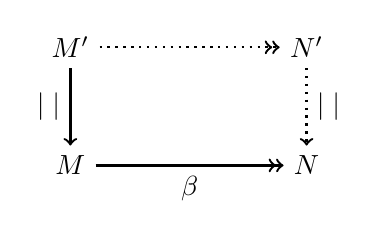
\begin{tikzpicture}[line width=0.3mm]
        \node(M') at (0,  0) {$M'$};
        \node(N') at (3,  0) {$N'$};
        \node(M)  at (0, -1.5) {$M$};
        \node(N)  at (3, -1.5) {$N$};

        \draw[->>, dotted] (M') edge node[above] {$\mbeta$} (N');
        \draw[->,  dotted] (N') edge node[right] {$|\;|$}   (N);
        \draw[->] (M') edge node[left] {$|\;|$}   (M);
        \draw[->>](M)  edge node[below] {$\beta$} (N);
      \end{tikzpicture}
      \end{center}

    \item $\forall m' \in \mlambda, m n \in \lambda, m' \xrightarrow{|\;|} m
      \wedge M \xrightarrow{\beta} N \Rightarrow \exists N' \in \Mlambda, M'
      \xrightarrow{\mbeta} N' \wedge N' \xrightarrow{|\;|} N$

      \begin{center}
      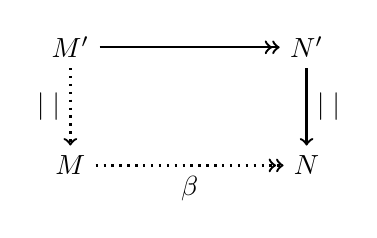
\begin{tikzpicture}[line width=0.3mm]
        \node(M') at (0,  0) {$M'$};
        \node(N') at (3,  0) {$N'$};
        \node(M)  at (0, -1.5) {$M$};
        \node(N)  at (3, -1.5) {$N$};

        \draw[->>] (M') edge node[above] {$\mbeta$} (N');
        \draw[-> ] (N') edge node[right] {$|\;|$}   (N);
        \draw[->,  dotted] (M') edge node[left]  {$|\;|$} (M);
        \draw[->>, dotted] (M)  edge node[below] {$\beta$} (N);
      \end{tikzpicture}
      \end{center}
  \end{enumerate}
  \textit{Proof}:
    \begin{enumerate}
      \item We proceed by induction on the reduction $M \rsbeta N$. 
        \begin{itemize}
          \item $M \rsbeta M$, then $M = N$. We just take $M' = M$ (easy).
          \item $M \rbeta M_t$ and $M_t \rsbeta N$. By induction hypothesis we
            have $M_t'$ such that $|M_t'| = M_t $ and $M_t' \rsbeta N'$.

            The reduction $M' \to_\mbeta M'_t$ exists, we can contract the same
            redex (if it was marked we would contract the new unmarked).

            So we have $M' \to_\mbeta M'_t \to_\mbeta N' \xrightarrow{|\;|} N$
        \end{itemize}
      \item Similar.
    \end{enumerate}
  \qedsymbol

  \lemma $\varphi$ property
    \label{lemm:phi}

    \begin{enumerate}
      \item $\forall u v \in \Mlambda, \varphi(u\{x \leftarrow v\}) =
        \varphi(u)\{x \leftarrow \varphi(v)\}$

      \item $\forall M N \in \Mlambda, M \tosmbeta N \Rightarrow \varphi(M)
        \rsbeta \varphi(N)$

        \begin{center}
        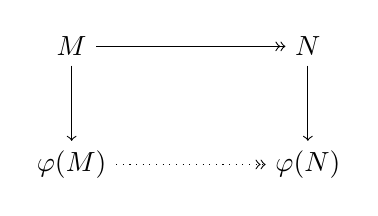
\begin{tikzpicture}
          \node(M)  at (0, 0) {$M$};
          \node(N)  at (3, 0) {$N$};
          \node(PM) at (0, -1.5) {$\varphi(M)$};
          \node(PN) at (3, -1.5) {$\varphi(N)$};

          \draw[->] (M) edge (PM) (N) edge (PN);
          \draw[->>] (M) edge (N);
          \draw[->>, dotted] (PM) edge (PN);
        \end{tikzpicture}
        \end{center}
    \end{enumerate}
    \textit{Proof}:
      \begin{enumerate}
        \item We proceed by induction on the term $u$.

          \begin{itemize}
            \item Case $u = z$
              \begin{itemize}
                \item if $z = x$, then
                  $\varphi(x\{x \leftarrow v\}) = \varphi(v) = \varphi(x)\{x
                  \leftarrow \varphi(v)\}$
                \item if $z \not = x$, then
                  $\varphi(z\{x \leftarrow v\}) = z = \varphi(z)\{x
                  \leftarrow \varphi(v)\}$
              \end{itemize}

            \item Case $t = \lambda y. t_0$,
              \begin{align*}
                \varphi((\lambda y. t_0)\{x \leftarrow v\})
                &= \varphi(\lambda y. t_0\{x \leftarrow v\}) \\
                &= \lambda y. \varphi(t_0\{x \leftarrow v\}) & \text{By
                convention} \\
                &= \lambda y. \varphi(t_0)\{x\leftarrow \varphi(v)\} & \text{By
                induction hypothesis} \\
                &= \varphi(\lambda y.t_0)\{x\leftarrow \varphi(v)\}
              \end{align*}

            \item Case $t = t_1\;t_2$
              \begin{align*}
                \varphi((t_1\;t_2)\{x \leftarrow v\})
                &= \varphi(t_1\{x \leftarrow v\}) (\varphi(t_2\{x \leftarrow v\})) \\
                &= \varphi(t_1)\{x \leftarrow \varphi(v)\} \varphi(t_2)\{x
                  \leftarrow \varphi(v)\}) & \text{By induction hypothesis}\\
                &= (\varphi(t_1)\;\varphi(t_2)) \{x \leftarrow \varphi(v)\}) \\
                &= (\varphi(t_1\;t_2)) \{x \leftarrow \varphi(v)\}) \\
              \end{align*}

            \item Case $t=(\mlambda y. t_0)\;t_1$
              \begin{align*}
                \varphi(((\mlambda y. t_0)\;t_1)\{x \leftarrow v\})
                &=\varphi((\mlambda y. t_0\{x \leftarrow v\})\;t_1\{x
                \leftarrow v\}) \\
                &=\varphi(t_0\{x \leftarrow v\})\{y\leftarrow \varphi(t_1\{x
                \leftarrow v\})\} \\
                &=\varphi(t_0)\{x \leftarrow \varphi(v)\})\{y\leftarrow
                \varphi(t_1)\{x \leftarrow \varphi(v)\}\} & \text{By induction
                hypothesis}\\
                &=\varphi(t_0)\{y\leftarrow \varphi(t_1)\}
                            \{x \leftarrow \varphi(v)\} & \text{By the lemma
                            \ref{exo:commsubst}}\\
                &=\varphi((\mlambda y. t_0)\; t_1)\{x \leftarrow \varphi(v)\}
             \end{align*}
          \end{itemize}
        \item By induction on $\tosmbeta$, using $(1)$
      \end{enumerate}
    \qedsymbol

  \newpage
  \lemma \label{lemma:bar-phi}
  $\forall t, |t| \rsbeta \varphi(t)$

  \begin{center}
  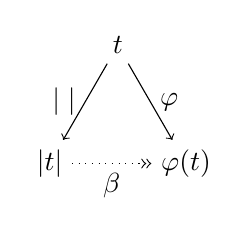
\begin{tikzpicture}
    \node(t) at (90:1) {$t$}; 
    \node(bt) at (210:1) {$|t|$}; 
    \node(pt) at (330:1) {$\varphi(t)$}; 

    \draw[->] (t) edge node[left] {$|\;|$} (bt)
              (t) edge node[right] {$\varphi$} (pt);
    \draw[->>, dotted] (bt) edge node[below] {$\beta$} (pt);
  \end{tikzpicture}
  \end{center}
  \textit{Proof}: We will show our property by induction on the term $t$.
  \begin{itemize}
    \item Case $t = x$, $|x| = x = \varphi(x)$, so we have $|t| \to_\beta^0
      \varphi(t)$.
    \item Case $t = \lambda x. t_0$, by the induction hypothesis we know that
      $|t_0| \rsbeta \varphi(t_0)$.
      \begin{align*}
        |(\lambda x. t_0)| &= \lambda x. |t_0| \\
        &\rsbeta \lambda x. \varphi(t_0) & \text{By induction hypothesis} \\
        &= \varphi(\lambda x. t_0)
      \end{align*}

    \item Case $t = t_1\; t_2$, by the induction hypothesis we know that
      $|t_1| \rsbeta \varphi(t_1)$ and $|t_2| \rsbeta \varphi(t_2)$.
      \begin{align*}
        |t_1\;t_2| &= |t_1|\;|t_2| \\
        &\rsbeta \varphi(t_1)\;\varphi(t_2) & \text{By induction hypothesis} \\
        &= \varphi(t_1\;t_2)
      \end{align*}

    \item Case $t=(\mlambda x. t_0)\;t_1$, by the induction hypothesis we know that
      $|t_0| \rsbeta \varphi(t_0)$ and $|t_1| \rsbeta \varphi(t_1)$.

        \begin{align*}
          |(\mlambda x. t_0)\;t_1| &= (\lambda x. |t_0|)\;|t_1| \\
            &\rsbeta (\lambda x. \varphi(t_0))\;\varphi(t_1) & \text{By
            induction hypothesis}\\
            &\to \varphi(t_0)\{x \leftarrow \varphi(t_1)\} \\
            &=\varphi((\mlambda x. t_0)\;t_1)
        \end{align*}

  \end{itemize}

  \qedsymbol

  \newpage
  \lemma Strip-lemma:

   $$\forall t\;t_1\;t_2, t \to t_1 \wedge t \to t_2 \Rightarrow \exists u, t_1
   \to^* u \wedge t_2 \to^* u$$

  \begin{center}
  \begin{tikzpicture}[line width=0.3mm]
    \node(t) at (0, 0) {$t$};
    \node(t1) at (-1, -1) {$t_1$};
    \node(t2) at ( 2, -1.5) {$t_2$};
    \node(u) at  ( 1,  -2.5) {$u$};

    \draw[->] (t) edge (t1);
    \draw[->>](t) edge (t2);
    \draw[dotted, ->>](t1) edge (u)
                      (t2) edge (u);
  \end{tikzpicture}
  \end{center}

  \textit{Proof}:
    Let $t'$, such that $|t'| = t$ and $\varphi(t') = t_1$. By hypothesis, we
    know that, $t \rsbeta t_2$, so we have by the Lemma-\ref{lemm:abs} $t_2' \in
    \Mlambda$ with $|t_2'| = t_2$. We take $u = \varphi(t_2')$.

    Then by the Lemma-\ref{lemm:phi}, we have
    $t_1 \rsbeta u$ and $\varphi(t_2') = u$. We finally have $t_2' \rsbeta u$
    thanks to the Lemma-\ref{lemma:bar-phi}.

    We can resume this proof with the diagram below:

    \begin{center}
    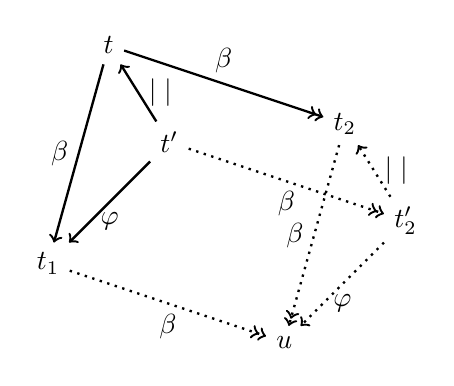
\begin{tikzpicture}[line width=0.3mm]
      \node(t)  at (0, 0, 0) {$t$};
      \node(t') at (0, -2,-2) {$t'$};
      \node(t1) at (0, -2, 2) {$t_1$};

      \node(t2)  at (3, -1, 0) {$t_2$};
      \node(t2') at (3, -3,-2) {$t_2'$};
      \node(u)   at (3, -3, 2) {$u$};

      \draw[->](t') edge node[right] {$|\;|$} (t)
               (t') edge node[below] {$\varphi$} (t1)
               (t)  edge node[left]  {$\beta$} (t1);
      \draw[->>](t) edge node[above] {$\beta$} (t2);
      \draw[->>, dotted] (t') edge node[below] {$\beta$} (t2');
      \draw[->>, dotted](t1) edge node[below] {$\beta$} (u);
      \draw[->>, dotted] (t2) edge node[left]  {$\beta$} (u);
      \draw[->,  dotted](t2')edge node[right] {$|\;|$}    (t2);
      \draw[->,  dotted](t2')edge node[below] {$\varphi$} (u);
    \end{tikzpicture}
    \end{center}

    Resume:
    \begin{enumerate}
      \item Lemma-\ref{lemm:abs}, give $t_2'$ : $t' \rsbeta t_2'$ and $|t_2'| =
        t_2$.
      \item Lemma-\ref{lemma:bar-phi}, give $t_2 \rsbeta \varphi(t_2') = u$.
      \item Lemma-\ref{lemm:phi}, give $t_1 \rsbeta \varphi(t_2') = u$
    \end{enumerate}

  \qedsymbol


  \subsubsection{Church-Rosser theorem}

  If $t_1 =_\beta t_2$ the there is $u$ such that $t_1 \to_\beta^* u$ and $t_2
  \to_\beta^* u$

  Consequences :

  \begin{itemize}
    \item if $t$ has a normal form $n$ then $t \to_\beta^* n$

    \item any $\lambda$-term can has only one normal form

    \item if two normal form $n$ and $m$ are syntactically different, then $n
      \not =_\beta m$.
  \end{itemize}




\end{document}
